\documentclass[12pt]{article}

\usepackage[utf8]{inputenc}
\usepackage[T2A]{fontenc}
\usepackage[english,russian]{babel}
\usepackage{graphicx}

\usepackage{titlesec}
\newcommand{\sectionbreak}{\clearpage}

\begin{document}

Title

\section*{Введение}

Темпоральная логика - это логика, учитывающая причинно-следственные связи в условиях времени.
Используется для описания последовательностей явлений и их взаимосвязи по временной шкале.
Темпоральные логики часто применяются для выражения требований формальной верификации.
Например, свойства типа «Если поступил запрос, то на него обязательно придёт ответ» или
«Функция вызывается не более одного раза за вычисление» удобно формулировать с помощью темпоральных логик.
В линейной темпоральной логике наряду с логическими операторами мы можем использовать следующие модальные операторы:
утверждение истинно в следующем состоянии, утверждение истинно всегда, утверждение когда-нибудь станет истинным,
одно утверждение будет истинным до тех пор пока другое утверждение не станет истинным,
одно утверждение не станет ложным до тех пор (включительно) пока другое не станет истинным.

Рассмотрим задачу нахождения формул линейной темпоральной логики, верных для заданного управляющего автомата.
Управляющий автомат характеризуется множествами состояний, входных воздействий и выходных воздействий,
а так же списком переходов, каждый из которых описывается начальным состоянием, конечным состоянием,
входным воздействием и множеством выходных воздействий. Таким образом базовыми утверждениями,
которые мы будем использовать являются следующие: произошло входное воздействие Е, произошло выходное воздействие А.
Интересовать нас будут не просто верные для автомата формулы, а те, на которые так же наложены некоторые
дополнительные требования. Во-первых мы хотим, чтобы сгенерированные формулы давали нам как можно больше информации
о входном автомате (в идеале полностью его описывали). Во-вторых генерируемые формулы предназначены для
использования людьми, а значит не должны быть слишком громоздкими. Позже эти требования будут формализованы.

Далее в работе будет рассмотренно решение этой задачи с помощью генетических алгоритмов - класса алгоритмов,
которые решают задачи оптимизации путем подбора параметров с использованием механизмов, аналогичных естественному
отбору в природе, - мутации, отбора и скрещивания.

\section*{1. Постановка задачи}

Пусть задан входной автомат. Требуется найти удовлетворяющие ему формулы, оптимальные в плане ранее указанных
двух соображений. Формализуем их.

Введем вес для базовых утверждений и операторов. Весом формулы будем называть будем называть следующее:
если формула является базовым утверждением, то это вес утверждения, если это оператор, то это вес оператора
плюс суммарный вес его аргументов. Будем искать формулы обладающие минимальным весом, формализовав таким
образом требование простоты формулы.

Рассмотрим множество автоматов, удовлетворяющих некоторой формуле. Будем считать, что чем меньше мощность
этого множества, тем больше информации о входном автомате несет формула.

\section*{2. Алгоритм}

Для решения задачи будем использовать генетический алгоритм. Будем преставлять формулу как ее дерево разбора.
Для генерации, скрещивания и мутации формул будем использовать стандартные алгоритмы генетического программирования,
описанные в книгах "Genetic programming I/II" (John Koza). Tак как в качестве целевых были выделены сразу несколько
критериев, то воспользуемся многокритериальной оптимизацией.

Многокритериальная оптимизация - это процесс одновременной оптимизации двух или более конфликтующих целевых функций
в заданной области определения. В качестве критерия оптимальности будем использовать оптимальность по Парето:
Говорят, что одно решение доминирует над другим, если оно по всем критерия не хуже другого и как минимум по одному
строго лучше. Множеством оптимальных решений называются решения, над которыми никто не доминирует. Таким образом
в качестве результата работы алгоритма будет получен фронт решений, являющихся оптимальными. Для реализации
многокритериальной оптимизации воспользуемся алгоритмом SPEA2.

В качестве критериев оптимизации будем использовать верность формулы для входного автомата, минимальность веса
формулы и минимальность числа автоматов, которым удовлетворяет формула. Очевидно, однако, что вычисление последнего
критерия не представляется возможным даже для небольшого числа состояний в автомате. Поэтому в дальнейшем будут
рассмотренны несколько критериев и их комбинаций, эффективно приближающих требуемое. Позже будет приведен
анализ качества их работы.

\subsection*{Критерий 1. Удовлетворение формулы входному автомату.}

Будем определять удовлетворяет ли формула автомату с помощью автомата Бюхи. При этом такая проверка будет возвращать
число из промежутка [0, 1] - отношение числа переходов, которым формула удовлетворяет, к общему числу переходов.
Таким образом если формула верна для автомата, то данная велечина будет равна еденице.

\subsection*{Критерий 2. Минимальность веса формулы.}

Пусть формула обладает неким весом w. Используем в качестве критерия велечину 1/w. Выберем в качестве весов числа не
меньше еденицы. В таком случае указанная велечина будет лежать в промежутке [0, 1].

\subsection*{Критерий 3. Число случайных автоматов, удовлетворяющих формуле.}

Сгенерируем некоторое число N случайных автоматов с теми же множествами состояний, входных и выходных событий, что и
у исходного. Для каждого из полученных автоматов измерим насколько формула ему уовлетворяет. Получим N чисел ci из
промежутка [0, 1]. В качестве результата возьмем велечину 1/(1 + r), где r - Евклидово расстояние в N-мерном
пространстве от 0 до c = <c1 ... cN>.

\subsection*{Критерий 4. Число мутантов исходного автомата, удовлетворяющих формуле.}

Возьмем исходный автомат и сгенерируем для него некоторое количество мутантов - исходных автоматов с небольшими
случайными изменениями. В качестве результата используем величину, аналогичную результату для случайных автоматов.

\subsection*{Критерий 5. Удовлетворение формулы автомату, построенному по сценариям.}

Сценарий - некоторый случайный путь в автомате фиксированной длинны. Построим для входного автомата некоторое
число сценариев. На основе этих сценариев построим новый автомат. Заметим, что полученный автомат будет удовлетворять
не всем формулам, верным для исходного автомата, так как длинна любого сценария конечна. В качестве результата используем
велечину 1 - с, где с - отношение чила удовлетворяющих формуле переходов к общему их числу.

\subsection*{Критерий 6. Число мутантов автомата, построенного по сценариям, удовлетворяющих формуле.}

Критерий аналогичен критерию номер четыре с тем лишь отличием, что мутанты строятся на основе автомата, построенного по
сценариям, а не исходного.

\section*{3. Результаты}

\subsection*{Проведенные испытания}

Для тестирования алгоритма использовался автомат, представленный на рисунке.

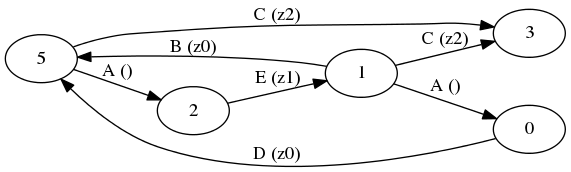
\includegraphics[scale=0.5]{lift.png}

Было проведено несколько запусков различных конфигураций алгоритма. Во всех конфигурациях использовались первые два критерия.
Для оставшихся четырех критериев были испытанны все комбинации. Всего таким образом было получено шестнадцать конфигураций.

Для оценки результатов наряду с простым анализом полученных формул будем использовать следующую велечину:
Построим на основе выведенных формул и сценариев автомат. Возьмем набор формул, написанных человеком для исходного автомата, и
проверим сколько из них удовлетворяют построенному автомату. Чем больше эта велечина, тем больше информации об исходном
автомате нам дают выведенные формулы.

\subsection*{Результаты испытаний}

Было проведено десять запусков каждой из шестнадцати конфигураций. Для входного автомата было написанно семнадцать формул.
Таким образом то, насколько много информации дают формулы, полученные с помощью некоторой конфигурации, о входном автомате,
характеризуется числом от 0 до 170.

Максимальный результат - 170 набрала реализация, в которой были использованны все критерии. Второе место с результатом 169
разделили две реализации: в обоеих не было критерия 5, в одной был использован 4, в другой нет. Третье место (164) так же
заняли две реализации: в первой былм использованны критерии 4, 5, во второй - 3, 5, 6. Далее приведены примеры сгенерированных
формул: 

G(F(wasAction(z1)) -> !wasAction(z2))

G(X(wasAction(z1)) -> wasEvent(A))

G(wasAction(z0) -> F(wasAction(z1) or X(wasAction(z2))))

G(X(wasAction(A)) -> (wasAction(z1) or wasAction(z0)))

\section*{4. Заключение}

Разработан метод генерации LTL-формул по конечному управляющему автомату и написана программа на языке программирования Java,
реализующая этот метод. Были протестированны различные конфигурации алгоритма и выбранны лучшие из них. При тестированнии
алгоритм показал достаточно стабильные результаты, было получено достаточное количество формул, удовлетворяющих поставленной цели.

\end{document}
